\section{Grundlagen}\label{sec:grundlagen}

\subsection{Business Process Identification}
\subsection{Methoden der Business Process Identification}

Die Identifikation von Geschäftsprozessen ist ein entscheidender Schritt für die Analyse, Modellierung und Optimierung von Geschäftsabläufen. Es gibt verschiedene Ansätze, um Geschäftsprozesse in einer Organisation zu identifizieren. In diesem Abschnitt wird eine Übersicht über die gängigsten Methoden gegeben.

\textbf{Interviews und Workshops:} Eine der häufigsten Methoden, um Geschäftsprozesse zu identifizieren, ist die Durchführung von Interviews und Workshops mit den beteiligten Stakeholdern. Durch diese direkte Interaktion können Informationen über die aktuellen Geschäftsabläufe, Herausforderungen und Verbesserungspotenziale gesammelt werden~\cite[5.2.2, 5.2.3]{Dumas2013}.

\textbf{Dokumentenanalyse:} Eine weitere Methode zur Identifikation von Geschäftsprozessen ist die Analyse von vorhandenen Dokumenten, wie z.B. Organigrammen, Verfahrensanweisungen, Arbeitsanweisungen und anderen relevanten Unterlagen. Diese Analyse ermöglicht es, einen Einblick in die Struktur und den Ablauf von Geschäftsprozessen zu gewinnen~\cite[5.2.1]{Dumas2013}.

\textbf{Observation:} Die Beobachtung von Mitarbeitern bei der Ausführung ihrer Aufgaben kann ebenfalls helfen, Geschäftsprozesse zu identifizieren. Diese Methode ermöglicht es, die tatsächlichen Abläufe und Interaktionen zwischen verschiedenen Abteilungen und Rollen in der Organisation zu verstehen.~\cite[5.2.1]{Dumas2013}

\textbf{Process Mining:} Process Mining ist eine datengetriebene Methode zur Identifikation von Geschäftsprozessen, bei der Ereignisprotokolle aus Informationssystemen analysiert werden. Mithilfe dieser Methode kann eine besonders gut skalierbare und wiederholbare Identifikation in großen Unternehmen und Abteilungen vorgenommen werden, wo andere Techniken oft zu Zeitintensiv wären.~\cite{Aalst2012}

In der Praxis wird häufig eine Kombination dieser Methoden verwendet, um ein umfassendes Verständnis der Geschäftsprozesse einer Organisation zu gewinnen und eine solide Grundlage für die weitere Analyse und Verbesserung zu schaffen.

\subsection{Business Process Identification durch Interviews}\label{subsec:interviews-grundlagen}
Interviews dienen als Methode zur Entdeckung von Geschäftsprozessen, indem die Beteiligten in die Prozessausführung einbezogen werden. Diese Technik hat ihre Vor- und Nachteile und kann in verschiedenen Phasen der Prozessentdeckung eingesetzt werden.

\textbf{Vorteile}

\begin{itemize}
    \item \textbf{Gründliche Informationen}: Interviews erleichtern die Sammlung detaillierter Informationen über Geschäftsprozesse, einschließlich der Perspektiven und Erfahrungen der Stakeholder~\cite{Dumas2013}.
    \item \textbf{Flexibilität}: Interviews können auf die Bedürfnisse und Perspektiven der Stakeholder zugeschnitten werden, so dass die Forscher die Fragen auf der Grundlage der Antworten der Teilnehmer anpassen können~\cite{Seidman2006}.
    \item \textbf{Validierung}: Interviews können dazu beitragen, Erkenntnisse aus anderen Datenquellen zu validieren und zu triangulieren, um ein umfassendes Verständnis der Prozesse zu gewährleisten~\cite{Denzin1978}.
    \item \textbf{Implizites Wissen}: Forscher können durch Interviews verstecktes oder implizites Prozesswissen aufdecken, einschließlich nicht dokumentierter Schritte oder informeller Praktiken~\cite{Dumas2013}.
\end{itemize}

\textbf{Nachteile}

\begin{itemize}
    \item \textbf{Subjektivität}: Interviews sind anfällig für Subjektivität und Voreingenommenheit, da die Teilnehmer unterschiedliche Perspektiven oder Interpretationen von Prozessen haben können~\cite{Seidman2006}.
    \item \textbf{Zeitaufwendig}: Die Durchführung und Auswertung von Interviews erfordert einen erheblichen Zeitaufwand für die Planung, Datentranskription und Analyse~\cite{Kvale2009}.
    \item \textbf{Geschränkte Verallgemeinerbarkeit}: Die Interviews werden mit kleineren Stichproben von Interessengruppen durchgeführt, was die Verallgemeinerbarkeit der Ergebnisse einschränken kann~\cite[P. 253]{Creswell2014}
    \item \textbf{Gedächtnis der Teilnehmer}: Interviews beruhen auf den Erinnerungsfähigkeiten der Teilnehmer, die durch Faktoren wie Zeit oder kognitive Verzerrungen beeinflusst werden können, was die Genauigkeit der bereitgestellten Informationen beeinträchtigt~\cite{Kvale2009}.
\end{itemize}

Interviews können in verschiedenen Phasen der Prozessentdeckung eingesetzt werden:

\begin{itemize}
    \item \textbf{Voruntersuchung}: Interviews können erste Informationen über Prozesse liefern, Beteiligte identifizieren und den Kontext für weitere Untersuchungen herstellen~\cite{Dumas2013}.
    \item \textbf{Verfeinerung von Prozessmodellen}: Nach der Erstellung von Prozessmodellen mit Hilfe anderer Methoden können Interviews dazu beitragen, diese Modelle zu validieren und zu verfeinern, indem Erkenntnisse der Stakeholder einbezogen werden und verstecktes oder implizites Prozesswissen aufgedeckt wird~\cite{Dumas2013}.
    \item \textbf{Evaluierung der Prozessleistung}: Mit Hilfe von Interviews lassen sich Rückmeldungen der Stakeholder zur Prozessleistung einholen, verbesserungswürdige Bereiche aufzeigen und potenzielle Lösungen untersuchen~\cite{Dumas2013}.
\end{itemize}

Zusammenfassend lässt sich sagen, dass Interviews eine wichtige Methode sind, um Geschäftsprozesse zu erforschen und zu verstehen, indem man sich mit Interessengruppen auseinandersetzt, die direkt an der Prozessausführung beteiligt sind. 

\subsubsection{Stakeholder-Kategorisierung}

Kategorisiere Stakeholder basierend auf ihren Rollen und Verantwortlichkeiten im Prozess.
Dies ermöglicht es dem Analysten, Fragen auf die spezifischen Bedürfnisse und Perspektiven jeder Gruppe zuzuschneiden, um eine umfassende und relevante Datenerhebung sicherzustellen\cite{Dumas2013}.

\subsubsection{Analysesziele definieren}

Skizziere die Ziele und Objektive der Analyse und identifiziere die spezifischen Aspekte des Prozesses, die untersucht werden sollen, sowie die Art der Informationen, die von jeder Stakeholder-Gruppe gesammelt werden sollen~\cite{Seidman2006}.

\subsubsection{Offene Fragen entwickeln}

Entwerfe offene Fragen, die detaillierte Antworten fördern und den Teilnehmenden ermöglichen, ihre Erfahrungen, Erkenntnisse und Meinungen zu teilen~\cite{Kvale2009}. 
Offene Fragen helfen, suggestive oder voreingenommene Fragen zu vermeiden, die die Antworten der Teilnehmenden beeinflussen könnten.

\subsubsection{Fokus auf den Prozess}

Stelle sicher, dass die Interviewfragen relevant für die Analysesziele sind und sich auf den Prozess selbst konzentrieren, einschließlich Input, Aktivitäten und Output sowie Faktoren, die den Prozess beeinflussen, wie Ressourcen, Werkzeuge, Technologien und Abhängigkeiten von anderen Prozessen~\cite{Dumas2013}.

\subsubsection{Nachfragen vorbereiten}

Entwerfe Nachfragen, um bestimmte Themen basierend auf der ursprünglichen Antwort des Teilnehmenden vertiefter zu untersuchen. Nachfragen helfen, Unklarheiten oder Inkonsistenzen in der ursprünglichen Antwort des Teilnehmenden zu klären und gewährleisten eine genaue und verlässliche Datenerhebung~\cite{Kvale2009}.

\subsection{Prozessmodellierung}\label{subsec:prozessmodellierung}
Aus den in der Business Process Discovery Phase gesammelten unstrukturierten Daten müssen in einem nächsten Schritt strukturierte Prozessmodelle erstellt werden, die als Grundlage für die weitere Analyse dienen.
Zur Modellierung von Geschäftsprozessen gibt es verschiedene Ansätze, die im Folgenden vorgestellt werden.

\subsubsection{UML}
Die Unified Modeling Language (UML) ist ein Standard für grafische Modellierung die für die Softwareentwicklung und das Systemdesign entwickelt wurde und die Darstellung und Dokumentation der Struktur und des Verhaltens von Systemen ermöglicht~\cite{OMG2017}.
Im Zusammenhang mit der Prozessmodellierung können im speziellen Aktivitätsdiagramme verwendet werden, um Prozesse in Aktionen aufgeteilt darzustellen, wobei verschiedene Akteure durch Swimlanes repräsentiert werden können~\cite{List2006}.\\

Allerdings hat die UML bei der Modellierung von Geschäftsprozessen gewisse Einschränkungen.
Während sie umfassende Unterstützung für Kontrollfluss- und Datenperspektiven bietet, ist ihre Anwendbarkeit auf ressourcenbezogene oder organisatorische Aspekte begrenzt~\cite{Russell2006}.
Darüber hinaus kann UML Schwierigkeiten haben, einige natürliche Konstrukte zu erfassen, die in Geschäftsprozessen vorkommen, wie z. B. Fälle und Interaktionen mit der betrieblichen Umgebung~\cite{Russell2006}.


\subsubsection{BPMN (Business Process Model and Notation)}

Die Business Process Model and Notation (BPMN) 2.0 ist eine standardisiertes Modellierungssprache, die verwendet wird, um Geschäftsprozesse grafisch darzustellen.
BPMN 2.0 wurde vom Object Management Group (OMG) entwickelt und bietet eine einheitliche Sprache, um Prozesse und Aktivitäten in Unternehmen zu beschreiben.\\
Das BPMN 2.0-Schema besteht aus einer Vielzahl von Symbolen, die zur Darstellung von Ereignissen, Aktivitäten, Gateways, Datenobjekten und weiteren Konstrukten verwendet werden.
Diese Symbole werden in einer grafischen Notation angeordnet, um einen Prozessfluss zu erzeugen, der die verschiedenen Schritte des Prozesses und deren Beziehungen zueinander widerspiegelt.

\begin{enumerate}[label=\arabic*., leftmargin=*]
    \item \textbf{Flow Objects}: Dies sind die wichtigsten grafischen Elemente, die zur Definition des Prozessverhaltens verwendet werden. Flow Objects werden in drei Typen unterteilt:
    \begin{enumerate}
        \item[] \begin{minipage}{\linewidth}
            \textbf{Events}: Kreise, die Ereignisse darstellen, die einen Prozess auslösen oder daraus resultieren können. Sie können Start-, Zwischen- oder Endereignisse sein.
            \begin{center}
                \begin{tikzpicture}[baseline=-0.5ex]
                    % Events
                    \node[draw, circle, minimum size=1cm] (start) {Start};
                    \node[draw, circle, double, minimum size=1cm, right=1cm of start] (intermediate) {Int.};
                    \node[draw, circle, minimum size=1cm, right=1cm of intermediate, line width=2pt] (end) {End};
                \end{tikzpicture}
            \end{center}
        \end{minipage}
    
        \item[] \begin{minipage}{\linewidth}
            \textbf{Activities}: Abgerundete Rechtecke, die die im Prozess ausgeführte Arbeit darstellen. Aktivitäten können Aufgaben oder Unterprozesse sein.
            \begin{center}
                
\begin{tikzpicture}[baseline=-0.5ex]
                    % Task
                    \node[draw, rectangle, rounded corners, minimum size=1cm] (task) {Task};
                    \end{tikzpicture}
            \end{center}
        \end{minipage}
        
        \item[] \begin{minipage}{\linewidth}
            \textbf{Gateways}: Rauten, die Entscheidungspunkte oder Gabelungen und Zusammenführungen von Pfaden im Prozess darstellen. Sie werden verwendet, um den Prozessfluss zu steuern.
            \begin{center}
                \begin{tikzpicture}[baseline=-0.5ex]
                    % Gateway
                    \node[draw, diamond, aspect=2, minimum size=1cm] (gateway) {};
                    \end{tikzpicture}
            \end{center}
        \end{minipage}
    \end{enumerate}

    \item \textbf{Verbindungsobjekte}: Dies sind die Elemente, die Flow-Objekte verbinden und die Reihenfolge des Prozesses oder des Nachrichtenflusses zwischen den Teilnehmern anzeigen. Zu den verbindenden Objekten gehören:
    \begin{enumerate}
        \item[] \begin{minipage}{\linewidth}
            \textbf{Sequence Flow:} Durchgehende Pfeile, die die Reihenfolge anzeigen, in der Aktivitäten, Ereignisse und Gateways ausgeführt oder ausgewertet werden.
            \begin{center}
            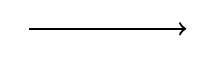
\begin{tikzpicture}[baseline=-0.5ex]
                % Sequence Flow
                \draw[->, thick] (0, 0) -- (2, 0);
            \end{tikzpicture}
            \end{center}
        \end{minipage}

        \item[] \begin{minipage}{\linewidth}
            \textbf{Message Flow:} Gestrichelte Pfeile, die den Austausch von Nachrichten zwischen den Teilnehmern eines Prozesses anzeigen.
            \begin{center}
                \begin{tikzpicture}[baseline=-0.5ex]
                    % Message Flow
                    \draw[dashed, ->] (0, 0) -- (2, 0);
                    \draw (0, 0) circle [radius=1.5pt];
                \end{tikzpicture}
                \end{center}
            \end{minipage}
        
        \item[] \begin{minipage}{\linewidth}
            \textbf{Association:} Gestrichelte Linien, die Daten, Anmerkungen oder Artefakte mit Flow-Objekten verbinden.
            \begin{center}
                \begin{tikzpicture}[baseline=-0.5ex]
                    % Association
                    \draw[dotted] (0, 0) -- (2, 0);
                \end{tikzpicture}
            \end{center}
        \end{minipage}
    \end{enumerate}

    \item \textbf{Swimlanes}: Diese Elemente werden verwendet, um den Prozess visuell zu organisieren und in verschiedene Rollen, Verantwortlichkeiten oder Funktionsbereiche zu unterteilen. Swimlanes umfassen:
    \begin{enumerate}
        \item[] \begin{minipage}{\linewidth}
            \textbf{Pools:} Rechtecke, die die an einem Prozess beteiligten Personen darstellen. Ein Pool kann eine oder mehrere Bahnen enthalten.
            \begin{center}
            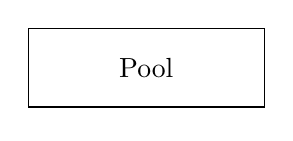
\begin{tikzpicture}[baseline=-0.5ex]
                % Pool
                \draw (0, 0) rectangle (3, 1);
                \node at (1.5, 0.5) {Pool};
            \end{tikzpicture}
            \end{center}
        \end{minipage}
        
        \item[] \begin{minipage}{\linewidth}
            \textbf{Lanes:} Unterabteilungen innerhalb eines Pools. Lanes helfen dabei, den Prozess auf der Grundlage von Rollen oder Funktionsbereichen innerhalb eines Teilnehmers weiter zu organisieren und zu kategorisieren.
            \begin{center}
            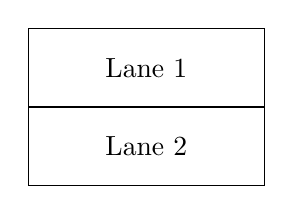
\begin{tikzpicture}[baseline=-0.5ex]
                % Lanes
                \draw (0, 0) rectangle (3, 2);
                \draw (0, 1) -- (3, 1);
                \node at (1.5, 1.5) {Lane 1};
                \node at (1.5, 0.5) {Lane 2};
            \end{tikzpicture}
            \end{center}
        \end{minipage}
    \end{enumerate}

    \item \textbf{Artifacts}: Diese Elemente liefern zusätzliche Informationen über den Prozess, die nicht direkt mit der Sequenz oder dem Nachrichtenfluss verbunden sind. Zu den Artefakten gehören:
    \begin{enumerate}
        \item[] \begin{minipage}{\linewidth}
            \textbf{Input Data Objects:} Icons, die Dateneingaben im Prozess darstellen.
            \begin{center}
                \begin{tikzpicture}[baseline=-0.5ex]
                    % Input Data Object
                    \draw (0, 0) -- (1, 0) -- (1, 1.3) -- (0.9, 1.4) -- (0, 1.4) -- (0, 0);
                    \node[single arrow, draw, minimum height=0.4cm, minimum width=0.4cm, anchor=west, yscale=0.4, single arrow head extend=0.1cm] at (0.1, 1.15) {};
                    \node at (0.5, 0.7) {IDO};
                \end{tikzpicture}
            \end{center}
        \end{minipage}
    
        \item[] \begin{minipage}{\linewidth}
            \textbf{Output Data Objects:} Icons, die Datenausgaben im Prozess darstellen.
            \begin{center}
                \begin{tikzpicture}[baseline=-0.5ex]
                    % Output Data Object
                    \draw (0, 0) -- (1, 0) -- (1, 1.3) -- (0.9, 1.4) -- (0, 1.4) -- (0, 0);
                    \node[single arrow, draw, minimum height=0.4cm, minimum width=0.4cm, anchor=west, yscale=0.4, single arrow head extend=0.1cm, fill=black] at (0.1, 1.15) {};
                    \node at (0.5, 0.7) {ODO};
                \end{tikzpicture}
            \end{center}
        \end{minipage}
    
        \item[] \begin{minipage}{\linewidth}
            \textbf{Data Stores:} Icons, die einen Ort darstellen, an dem Daten während der Prozessausführung gespeichert und abgerufen werden können.
            \begin{center}
            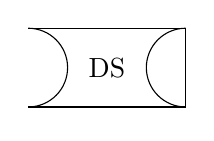
\begin{tikzpicture}[baseline=-0.5ex]
                % Data Store
                \draw (0, 0) -- (2, 0) -- (2, 1) -- (0, 1);
                \draw (0, 1) arc (90:-90:0.5);
                \draw (2, 1) arc (90:270:0.5);
                \node at (1, 0.5) {DS};
            \end{tikzpicture}
            \end{center}
        \end{minipage}
    
        \item[] \begin{minipage}{\linewidth}
            \textbf{Group:} Ein gestricheltes Rechteck, das Elemente des Prozesses visuell gruppiert und oft zu Dokumentationszwecken verwendet wird.
            \begin{center}
            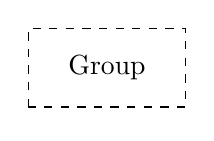
\begin{tikzpicture}[baseline=-0.5ex]
                % Group
                \draw[dashed] (0, 0) rectangle (2, 1);
                \node at (1, 0.5) {Group};
            \end{tikzpicture}
            \end{center}
        \end{minipage}
    
        \item[] \begin{minipage}{\linewidth}
            \textbf{Text Annotations:} Eine Klammer, die es ermöglicht Kommentare oder Beschreibungen zu jedem Teil des Prozesses hinzuzufügen.
            \begin{center}
            
\begin{tikzpicture}[baseline=-0.5ex]
                % Text Annotation
                \draw[decorate, decoration={brace, amplitude=5pt, mirror}] (0, 0) -- (0, 1);
                \node[anchor=west] at (0.2, 0.5) {Annotation};
            \end{tikzpicture}
            \end{center}
        \end{minipage}
    \end{enumerate}
\end{enumerate}

\subsubsection{Event-driven Process Chain (EPC)}
EPC ist ein Prozessmodellierungskonzept, das auf der Idee basiert, dass Prozesse aus einer Reihe von Ereignissen und Funktionen bestehen.
EPCs bieten eine grafische Darstellung, die es erlaubt, den Prozessfluss auf eine visuelle und verständliche Art darzustellen.
Die Methode wird häufig eingesetzt, da sie es ermöglicht, die Abhängigkeiten zwischen Prozessschritten einfach abzubilden und somit die Identifikation von Engpässen und Schwachstellen zu erleichtern.

\subsubsection{Fazit}
Die oben vorgestellten Modellierungssprachen sind alle auf die Darstellung von Geschäftsprozessen anwendbar. Allerdings unterscheiden sie sich in ihrer Herangehensweise, ihren Möglichkeiten und ihrem ursprünglichen Anwendungsgebiet.
Eine Literaturrecherche ergibt keine klare Empfehlung für eine der vorgestellten Sprachen, und ist selbst in direkten Vergleichen unterschiedlicher Sprachen gespaltener Meinung.
Die weitverbreitetste Sprache ist allerdings BPMN, weshalb sie im Rahmen dieser Arbeit genutzt wird.~\cite{Peixoto2008, Niziol2021}

\subsection{Anforderungsanalyse}\label{subsec:anforderungsanalyse-grundlagen}
Erläuterung des Begriffs Anforderungsanalyse aufzeigen verschiedener Methoden und Modellierungstechniken
